\section{Influences In Play}
Though the large amount of possibilities inherent in \emph{Sanguine Dreams}' Influences system can be daunting, 
the actual week to week submission of actions and results is very straightforward. This section details how best 
to post your Influences, the format of the response, and how multi-cycle actions resolve.

\subsection{How to Submit Influences}
Influence actions should always be submitted in writing, ideally using the ``Influences'' forum on our message boards.  
The submission should include how many points you are allocating to which action, whether or not you are using 
\emph{Contacts}, and clearly state what your goals are in the case of \emph{Endeavors}.  All actions which require a 
target should have it clearly labeled to reduce confusion. 

Influences are resolved in two-week cycles, with actions normally being due and results returned on alternating 
Wednesdays, via the message board.  Please do not submit actions for a future cycle until current results have 
been posted. \\

\noindent\textbf{Sample Influence Submission:}

\begin{quote}
	\textbf{Bureaucracy:} Endeavor x3 (I'm trying to close the Santa Rosa Safeway) \\
	\textbf{Finance:} Endeavor x1 (Raise \$1,000), Watch x2 (including 1 Contact) \\
	\textbf{Street:} Conceal x1 (last Cycle's Watch), Defend x1 (last Cycle's Endeavor), Watch x1 \\
	\textbf{University:} Follow x1 (Amanda), Follow x1 (Stephen), Growth x1
\end{quote}

\noindent Following the above example when making your posts greatly helps the Storytellers keep everything straight; every 
cycle there are hundreds of Influence actions submitted and every bit of uniformity helps reduce mistakes in a big way.

\subsection{Your Influence Results}
Taking the above example, let's look at the kind of results that character could receive for Finance.  First we'll 
see the information the Storyteller gave them and then explain what each result represents.

\begin{quote}
	\textbf{Finance --- Cycle 1} \\
	You have 2 dots +2 banked Growth actions \\
	This Influence is capped for level 5 -- nobody at level 4 can advance!  \\
	
	You observed the success of 2 Growth actions and the start of 3 more \\
	There are 3 other Watchers of this Influence  \\
	Someone is Combining their Influence with another \\
	You are attempting to: Raise \$1,000 \\
	Someone succeeded at:  Hire staff for a local restaurant \\
	Someone is attempting to:  Purchase a large business \\
	Someone Followed you!
\end{quote}

\noindent Every Influence result will begin with how many dots of a given sphere you have and how many banked 
\emph{Growth} actions you have.  Note that this count will not include any \emph{Growth} actions currently 
in-progress---it only lists those which have already succeeded.  You will also learn whether or not a 
particular sphere is capped, meaning there's no more room at a particular level.  Influence Caps are explained 
more fully in the next section.

The next lines show the results of the character's \emph{Watch} action; they get a detailed list of how many 
\emph{Growth} actions succeeded and began this cycle, how many other people were \emph{Watching} this Influence, 
and then the details of other actions.  Because this character was \emph{Watching}, they learned that someone 
\emph{Followed} them this cycle, something they may want to investigate later.

Now that this character has observed all of these actions, their options really expand for next cycle.  They could 
\emph{Trace} any of the actions they saw, \emph{Attack} anything currently in-progress, or use their points to 
\emph{Defend}, \emph{Conceal}, or \emph{Stealth} their own actions during next cycle.  The possibilities are 
endless!

\subsection{Working with Multi-Cycle Actions}
Some Influence actions, particularly \emph{Endeavor}, \emph{Growth}, and \emph{Kill}, take more than one cycle to 
complete.  To understand how these particular actions resolve, please see the following example, where a new 
\emph{Endeavor} is started in each of three cycles: \\

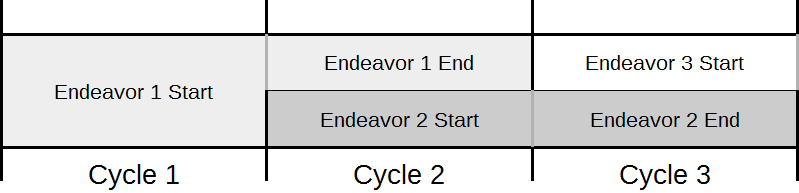
\includegraphics[width=0.9\linewidth]{MultiCycle.png}

\noindent Points are only spent to start each of the above actions; unless stopped (say by an \emph{Attack} action) they will 
conclude at the end of the next subsequent cycle.  This figure illustrates how points spent in Cycle 1 to start an 
action are again available in Cycle 2, even if the action itself hasn't completed yet.  Instead of starting a new 
\emph{Endeavor} these points could be spent on any type of action, including \emph{Defending} or \emph{Stealthing} 
the action started in the previous cycle.

Actions that have just started will show up under \emph{Watch} results as ``Someone is attempting to \ldots'' while actions 
which have concluded will return ``Someone has successfully \ldots'' or ``Someone has failed to \ldots''.  Note that if either 
the start or end of a multi-cycle action is \emph{Stealthed}, it won't appear on that cycle's results unless countered by a 
superior \emph{Watch}, as described in the Actions section.

\subsection{Absence and Influence Erosion}
Like so much else in life, Influences adhere to the adage of ``if you don't use it, you lose it.''  Those characters who have 
let their Influences lay idle for four consecutive cycles (at least two real-world months!) may find that they are subject 
to \emph{Erosion}, a special kind of action which emulates \emph{Kill} and can only be countered by putting your Influences back 
to work.  Idle Influences will be suffer one \emph{Erosion} action per cycle, which will be visible to anyone \emph{Watching} that 
sphere.

Unless a particular sphere is heavily impacted, the Storytellers generally only enforce \emph{Erosion} actions against those with 
level 4 and 5 Influences---the the levels in which most spheres have limited capacity and people actively jockeying for position.  
In all cases players will be given ample warning about the impending or continuing \emph{Erosion}, normally through the game's 
online message board.
